\begin{surferIntroPage}{Suprafe\c{t}e record mondial}{record_chmutovoktic}{Suprafe\c{t}e record mondial}

      O suprafa\c{t}\u{a} se nume\c{s}te \emph{nesingular\u{a}} sau \emph{neted\u{a}} daca nu are v\^{a}rfuri (astfel de puncte se numesc
      \emph{singularit\u{a}\c{t}i}). Exemple de suprafe\c{t}e netede sunt sfera sau torul (vezi primele doua figuri de mai jos).
      O suprafa\c{t}\u{a} aleas\u{a} aleator va fi aproape sigur nesingular\u{a}.

 \begin{center}
      \vspace{-0.2cm}
      \begin{tabular}{@{}c@{}c@{}c@{\quad}c@{}c@{}c@{}c@{}}
        \begin{tabular}{@{}c@{}}
          neted\u{a}:
        \end{tabular}
        &
        \begin{tabular}{@{}c@{}}
          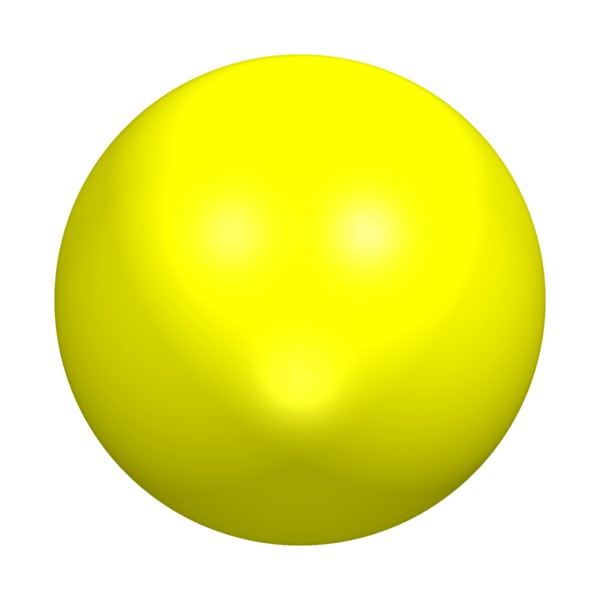
\includegraphics[width=1.1cm]{kugel}
        \end{tabular}
        &
        \begin{tabular}{@{}c@{}}
          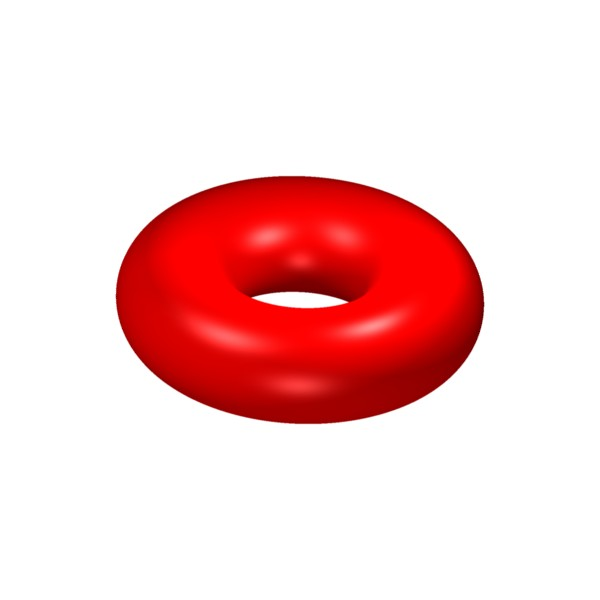
\includegraphics[width=1.1cm]{torus}
        \end{tabular}
        &
        \begin{tabular}{@{}c@{}}
          multe\\
          singularit\u{a}\c{t}i:
        \end{tabular}
        &
        \begin{tabular}{c@{}@{}}
          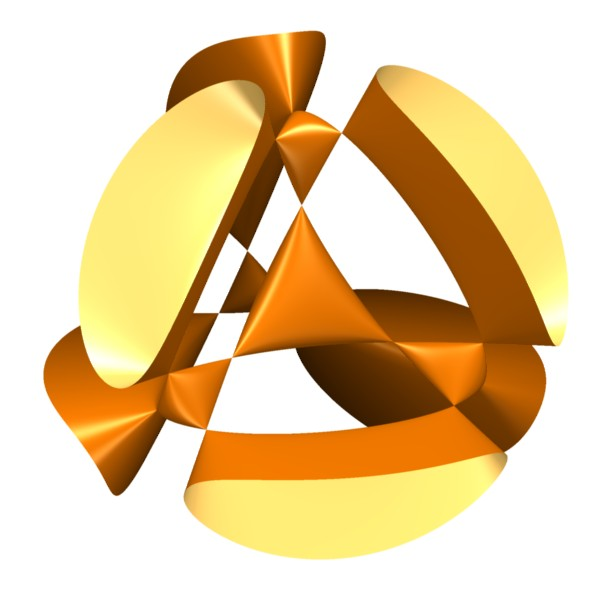
\includegraphics[width=1.1cm]{kummer}
        \end{tabular}
        &
        \begin{tabular}{c@{}@{}}
          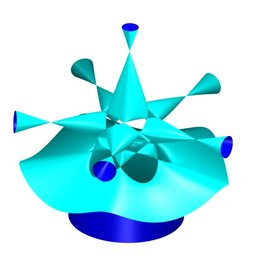
\includegraphics[width=1.1cm]{togliatti}
        \end{tabular}
        &
        \begin{tabular}{c@{}@{}}
          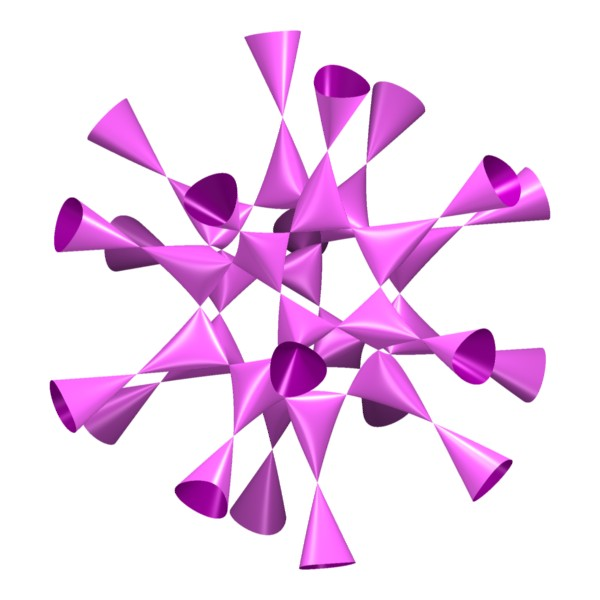
\includegraphics[width=1.1cm]{barth_sextic}
        \end{tabular}
      \end{tabular}
    \end{center}
    \vspace{-0.2cm}
            Astfel, este foarte special atunci c\^{a}nd o suprafa\c{t}\u{a} admite singularit\u{a}\c{t}i. Acestea sunt cele mai interesante puncte ale unei suprafe\c{t}e.
        Suprafe\c{t}ele din programele SURFER sunt definite de polinoame. Cea mai mare putere dintr-un polinom se nume\c{s}te gradul polinomului,
        notat $d$. Matematicienii vor \^{i}ntreba c\^{a}t de multe singularit\u{a}\c{t}i poate avea o suprafa\c{t}\u{a} de grad dat.
        Vom nota acest num\u{a}r cu $\mu(d) $.

   Se dovede\c{s}te c\u{a} acest num\u{a}r $\mu(d)$ este foarte greu de calculat.
   Valoarea lui $\mu(d)$ pentru $d=1,2,3,4$ era cunoscuta inc\u{a} din secolul XIX,
   pentru $d=5$ valoarea a fost identificat\u{a} \^{i}n 1980, \c{s}i pentru $d=6$ \^{i}n 1996.
   Pentru $d\ge 7$, $\mu(d)$ nu se cunoa\c{s}te \^{i}nc\u{a}.

   A\c{s}adar, fiecare nou record mondial pentru un $\mu(d)$ este un rezultat par\c{t}ial important.
   Se pare ca va lua mult timp p\^{a}n\u{a} c\^{a}nd problema va fi rezolvat\u{a} complet pentru $d$
   arbitrar. Iat\u{a} c\^{a}teva rezultate cunoscute:

   \begin{center}
      \begin{tabular}{r|cccccccc|c}
        $d$ & $1$ & $2$ & $3$ & $4$ & $5$ & $6$ & $7$ & $8$ & $d$\\
        \hline
        \hline
        \rule{0pt}{1.2em}$\mu(d)\ge$ & $0$ & $1$ & $4$ & $16$ & $31$ & $65$ &
        $99$ & $168$ &
        $\approx \frac{5}{12}d^3$\\[0.3em]
        \hline
        \rule{0pt}{1.2em}$\mu(d)\le$ & $0$ & $1$ & $4$ & $16$ & $31$ & $65$ &
        $104$ & $174$ & $\approx \frac{4}{9}d^3$
      \end{tabular}
    \end{center}
\end{surferIntroPage}
